\section{Internetová reklama}\label{sec:online-ad}
Moderní digitální doba nabízí mnoho způsobů, kterými lze komerční sdělení šířit. Jako jedny z hlavních forem se stává grafická (display) reklama,
reklama ve vyhledávání a emailech. Nejčastějšími poskytovateli se staly sociální sítě a vyhledávače.
Obrovské množství denních uživatelů z nich udělali perfektní platformy pro nabízení inzercí.
Obrázek \ref{fig:spir-publishers} a tabulka \ref{tab:spir-publishers} zobrazují srovnání návštěvnosti 5 největších poskytovatelů online reklamy v České republice.

\begin{figure}[h]
    \centering
    \caption[Graf návštěvosti provozovatelů reklamních sítí]{Graf návstěvnosti reálných uživatelů provozovatelů reklamních sítí v ČR \cite{gemius:rating}}
    \label{fig:spir-publishers}
    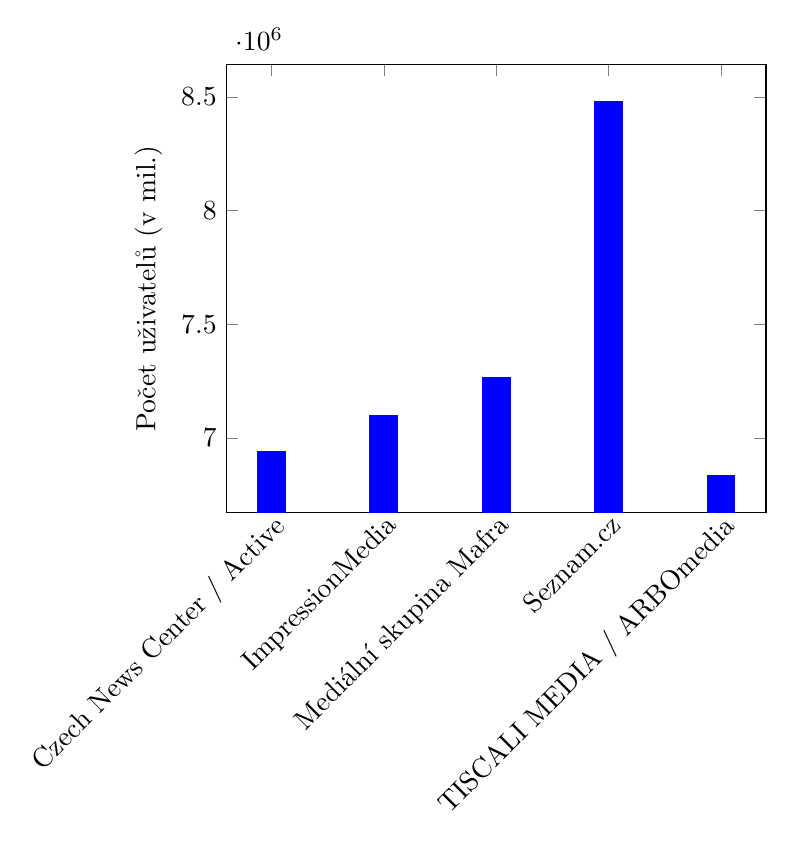
\begin{tikzpicture}
        \begin{axis}[
            symbolic x coords={Czech News Center / Active, ImpressionMedia, Mediální skupina Mafra, Seznam.cz, TISCALI MEDIA / ARBOmedia },
            x tick label style={rotate=45, anchor=north east, inner sep=0mm},
            xtick=data,
            ylabel=Počet uživatelů (v mil.),
          ]
            \addplot[ybar, fill, blue] coordinates {
                (Czech News Center / Active, 6938568)
                (ImpressionMedia,            7100320)
                (Mediální skupina Mafra,     7266377)
                (Seznam.cz,                  8480248)
                (TISCALI MEDIA / ARBOmedia,  6836590)
            };
        \end{axis}
    \end{tikzpicture}
    
\end{figure}

\begin{table}[hb]
    \centering
    \caption[Srovnání provozovatelů reklamních sítí]{Srovnání provozovatelů reklamních sítí \cite{gemius:rating}}
	\label{tab:spir-publishers}
    \begin{tabular}{l|r|r|r|r}
        \toprule
            Název & Reální uživatelé & Zobrazení stránky & Návštěvy & Čas \\
        \midrule
            Seznam.cz & 8 480 248 & 4 541 397 144  & 1 104 367 612 & 13782r 58d  \\
            Mediální skupina Mafra & 7 266 377 & 741 803 207  & 128 011 647  & 1156r 302d \\
            ImpressionMedia & 7 100 320  & 258 039 333 & 91 386 082 & 370r 7d  \\
            Czech News Center / Active & 6 938 568 & 508 776 721 & 110 070 333  & 549r 310d  \\
            TISCALI MEDIA / ARBOmedia & 6 836 590 & 120 326 836  & 44 648 445 & 204r 83d  \\
        \midrule
        
    \end{tabular}
\end{table}


Co se týče emailové reklamy, považuje se efektivní formu přímého marketingu, která je navíc zdarma.
Umožňuje firmám komunikovat se svými zákazníky jakožto stálými odběrateli nebo mají možnost rozesílat hromadné emaily. Legislativně je však nevyžádaná elektronická pošta ošetřena.
Firmy si tedy při rozesílání emailů musí být jisté, že je jejich sdělení oprávněné a nebude označeno jako spam.

Reklama ve vyhledávání se stává již placenou, většinou stylem PPC. Zadavatelé se za příplatek dostanou na první pozice výsledku hledání.
Toto jim zajišťuje vyšší míru prokliků a lépe nalákají potenciální zákazníky na svou webovou stránku.
Pro jakousi optimalizaci zobrazení reklamy si inzerent může vybrat, zda zvolí více obecnější nebo specifická klíčová slova pro svůj produkt/službu. Tyto strategie se anglicky označují
jako \emph{\enquote{head term}} (obecná klíčová slova) a \emph{\enquote{long tail}} (specifická klíčová slova) \cite{ads:long-tail}.
Pokud je využita strategie head term, reklama se zobrazí většímu množství
uživatelů vyhledávače, zatímco long tail zajistí relevantnější potenciální zákazníky.

Grafická reklama (nejčastěji bannery a videa) je silným nástrojem pro rozšíření působnosti značky. Buduje povědomí o značce a
zároveň může lákat na produkt. Obsahuje reklamní sdělení, logo firmy a výzvu k akci (CTA) -- nejčastěji ve formě tlačítka.
Obrázek \ref{fig:spir-ad-performance} Ukazuje srovnání investic do grafické a vyhledávané reklamy.

\begin{figure}[h]
    \centering
    \caption[Výkon reklam v roce 2020]{Výkon jednotlivých forem internetové reklamy v roce 2020 \cite{spir:mediatypes}}
    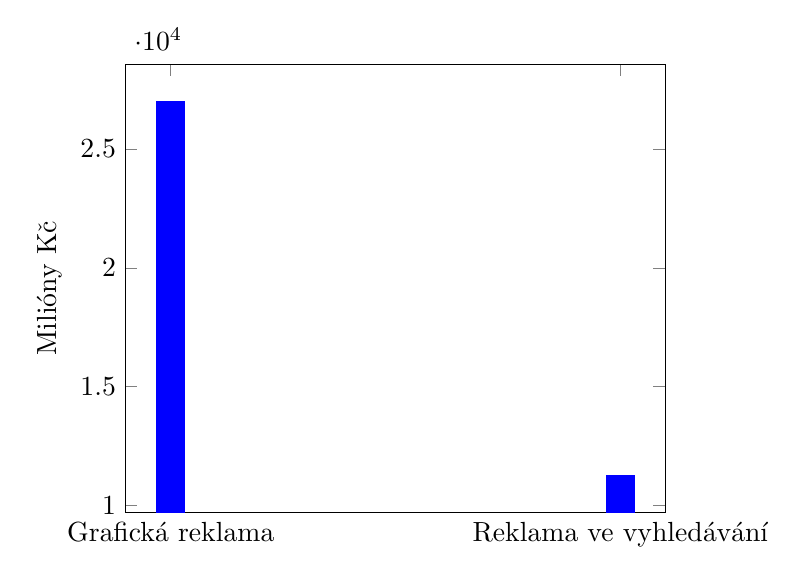
\begin{tikzpicture}
        \begin{axis}[
            symbolic x coords={Grafická reklama, Reklama ve vyhledávání},
            xtick=data,
            ylabel=Milióny Kč
          ]
            \addplot[ybar, fill, blue] coordinates {
                (Grafická reklama,           26998)
                (Reklama ve vyhledávání,     11274)
            };
        \end{axis}
    \end{tikzpicture}
    \label{fig:spir-ad-performance}
\end{figure}

    \subsection{Metriky internetových reklam}\label{ssec:online-ad-metrics}
    Jak tato práce již zmiňovala, výhodou online inzercí je jejich jednoduchý monitoring. Na rozdíl od ostatních médií si firmy mohou být více jisté,
    že jejich reklamu cílené osoby opravdu vnímají. Hlavní metrikou reklamy vždy bývá zvýšení prodeje.
    Nicméně tato metrika se měří obtížně a je spíše výsledkem níže uvedených následujících ukazatelů.

        \subsubsection{Míra prokliku (CTR)}
        Takzvaná míra prokliku určuje, jak je velká šance, že na reklamu někdo zareaguje kliknutím myši. Určuje se poměrem mezi celkovým počtem zobrazení reklamy a
        kliknutím na ni. Význam této metriky spočívá v tom, že dokáže prozradit úspěšnost kampaně z hlediska upoutání pozornosti.

        \subsubsection{Míra okamžitého opuštění (BCR)}
        Tento ukazatel zaznamenává procento uživatelů, kteří se vlivem reklamy dostali na cílovou webovou stránku, ale neprovedou žádnou další aktivitu a
        typicky z webu odejdou. Vysoká procento BCR nejčastěji indikuje jednu z následujících věcí:
        \begin{itemize}
            \item Cílová webová stránka byla nízké kvality -- nezajímavý vzhled, nepřístupnost, dlouhá doba načítání atd.
            \item Produkt nebo služba nabízená v reklamě nesouvisí s tím, co člověk hledal.
            \item Osoba na stránce našla vše potřebné a další informace nepotřebuje.
        \end{itemize}

        \subsubsection{Konverzní poměr (CVR)}
        Konverzní poměr je výsledkem součtu osob, kteří se skrze reklamu dostali na webovou stránku, dokončili nějakou akci (a stali se tak zákazníky) s
        celkovým počtem zobrazení stránky. Akci, kterou mají uživatelé splnit, si firma určí sama. Pro e-shopy toto může znamenat dokončení objednávky,
        pro blogy třeba přehlášení k newsletteru. Samotná cesta zákazníka od prvního zhlédnutí reklamy po dokončení akce může být dlouhý proces. Internetová
        reklama má převážně za úkol potenciálního zákazníka přivést na web, který ostatními marketingovými a vizuálními argumenty přesvědcí tohoto diváka například
        ke koupi daného zboží.

        \subsubsection{Návratnost investic (ROI)}
        Inzerování je spjato s náklady a investicí. Ve své nejjednodušší podstatě je poměr nákladů a výdělku výslednou metrikou.
        Výdělkem však nemusí být pouze zisk, ale i jiný cíl, který si firma stanoví (zvýšení popularity, uživatelů atd.).

    \subsection{Zobrazení online reklamy}
    Pro dobré využití reklamy je potřebné ji umístit na dobře viditelná místa webových stránek s vysokou návštěvností.
    Dnes jsou nejvíce navštěvované převážně sociální sítě typu Facebook, Youtube, Twitter apod. Jelikož tito giganti vlastní i více dalších podobných stránek,
    vznikly reklamní sítě jako Google Ads. To umožnilo vznik partnerských webů, které zobrazují reklamy právě prostřednictvím těchto sítí.
    Na oplátku dostávají partnerské weby část tržby ze zobrazených inzercí.

    Zmiňované reklamní sítě mají za úkol umístit správnou reklamu na správný web.
    Korektní stránku lze vybrat na základě jejího celkového obsahu, klíčových slov vyhledávání spotřebitele či dokonce z analýzy způsobu prohlížení stránky.
    Dá si říci, že inzerenti si kupují \enquote{online prostor} pro svou reklamu. 

    Druhou možností je \enquote{kupovat} si cílové publikum své reklamy prostřednictvím aukce, a to za pomocí technologie \emph{RTB}.
    Na začátku tvorby reklamní kampaně si inzerent vybere svou cílovou skupinu. Tu specifikuje pomocí různých demografických kritérií.
    Ve zjednodušené podobě je průběh RTB znázorněn na obrázku \ref{fig:rtb}.

    \begin{figure}[h]
        \centering
        \caption[Fungování RTB]{Zjednodušený způsob fungování RTB \cite{rtb}}
        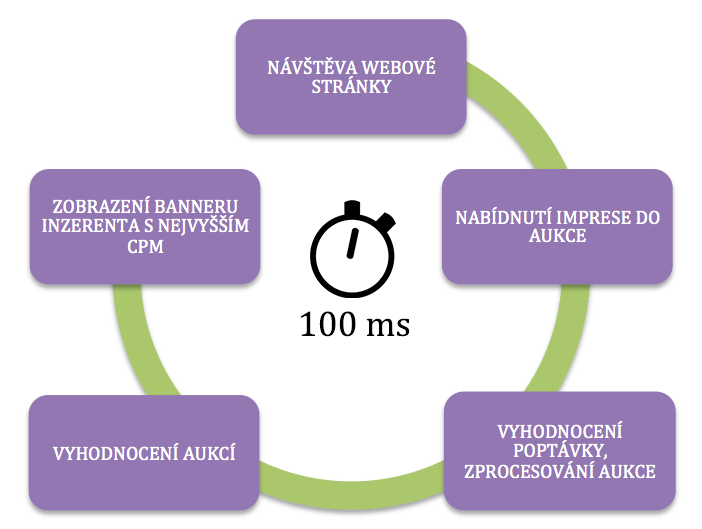
\includegraphics[width=0.7\textwidth]{Figures/rtb.png}
        \label{fig:rtb}
    \end{figure}

\endinput